\scanpage{72}\mspage{71}

Pour la suite, il faut faire attention si les axiomes vont passer aux sous-contrées. Introduisons quand $==$ la définition en forme

% figure: pleine-leader. The raised phrase and its hooked leader occur once.
\figure{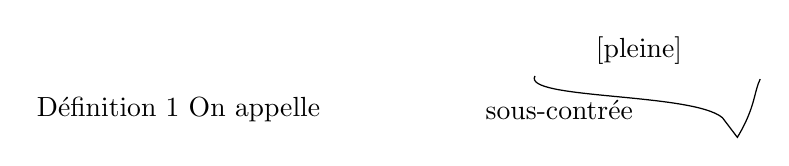
\begin{tikzpicture}[x=1cm,y=1cm]
\node[anchor=west] at (0,0) {\uline{Définition 1} On appelle};
\node[anchor=west] at (5.7,0) {\uline{sous-contrée}};
\node[anchor=west] at (7.1,.75) {\inserted{[\uline{pleine}]}};
\draw[line width=.45pt] (6.45,.43) .. controls (6.28,.13) and (8.45,.22) .. (8.83,-.10) -- (9.02,-.35) .. controls (9.25,.03) and (9.23,.23) .. (9.31,.39);
\end{tikzpicture}}
de la contrée $\unsure{\rlap{$\deleted{\mathcal F}$}\mathcal C|\mathscr C|\mathbb C}=(\mathcal F,\leq,\preceq)$, \unsure{tout|\deleted{tout}} sous-ens. qui \unsure{satisfont|satisfait} les conditions

a) fermé pour $\leq$, et stable par sup quelc. pour $\leq$ [et à ce titre, s'en correspond,
% figure: a-insertion-leaders. Both raised additions and the associated strokes.
\figure{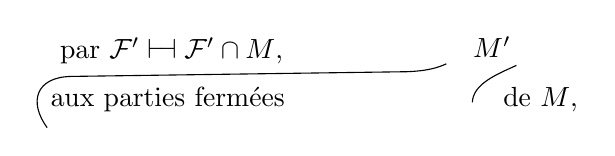
\begin{tikzpicture}[x=1cm,y=1cm]
\node[anchor=west] at (0,0) {aux parties fermées};
\node[anchor=west] at (5.75,0) {de $M$,};
\node[anchor=west] at (.12,.62) {\inserted{par $\mathcal F'\mathrel{\vdash\joinrel\dashv}\mathcal F'\cap M$,}};
\draw[line width=.4pt] (.08,-.36) .. controls (-.16,-.03) and (-.06,.28) .. (.38,.29) -- (4.65,.35) .. controls (4.91,.36) and (5.04,.40) .. (5.15,.45);
\node at (5.73,.66) {\inserted{$M'$}};
\draw[line width=.4pt] (5.48,-.04) .. controls (5.49,.20) and (5.80,.32) .. (6.04,.43);
\end{tikzpicture}}
par $M'\unsure{\mathrel{\mapstochar\relbar}|\mapsto|\mathrel{\vdash\joinrel\dashv}}\mathcal F'=\{F\in\mathcal F\mid\overline F\subset M'\}$].

% slanted
\margin{Je ne sais s'il faut prendre des sup quelconques (\unsure{condition} stricte) \deleted{\unsure{et}} ou bien de sup finis seulement \unsure{(condition lge|(condition large|(condition lge)|(condition large)}}

b) fermé pour $\preceq$ (ce qui impose une restriction aux parties envisagées $M'$ de $M$\unsure{\}|?}, \deleted{\unsure{savoir|à savoir} : si $X\in$} \inserted{qu'on va formuler} plus bas)

% figure: marginal-c. The note lies above C6 at the right; the pointer is drawn.
\figure{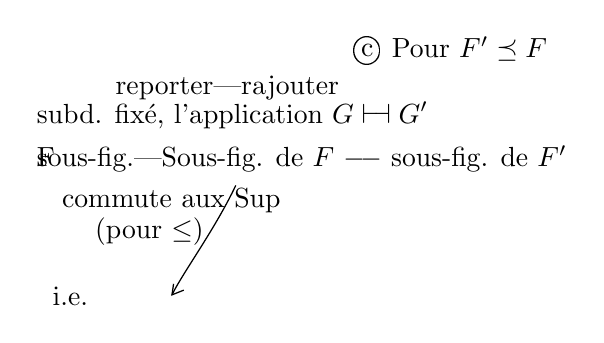
\begin{tikzpicture}[x=1cm,y=1cm]
\node[anchor=west] at (1.0,.35) {\unsure{reporter|rajouter}};
\node[anchor=west] at (4.0,.82) {\textcircled{c} Pour $F'\preceq F$};
\node[anchor=west] at (0,0) {subd. fixé, l'application $G\mathrel{\vdash\joinrel\dashv}G'$};
\node[anchor=west] at (0,-.55) {\unsure{\rlap{\deleted{F}}sous-fig.|Sous-fig.} de $F$ $\mathrel{\relbar\joinrel\relbar}$ sous-fig. de $F'$};
\node[anchor=west] at (.32,-1.08) {commute aux Sup};
\node[anchor=west] at (.74,-1.48) {(pour $\leq$)};
\node[anchor=west] at (.20,-2.30) {i.e.};
\draw[line width=.45pt] (2.65,-.89) .. controls (2.39,-1.44) and (1.97,-2.01) .. (1.84,-2.28);
\draw[line width=.45pt] (1.86,-2.14) -- (1.84,-2.28) -- (1.99,-2.22);
\end{tikzpicture}}

% diagram: C6-group. Diagrams remain diagrams; the two side rules, detached
% points and oblique gloss keep their relative positions. No text is repeated.
\diagram{\begin{tikzpicture}[x=1cm,y=1cm]
\node[anchor=west] at (0,0) {\uline{C6}};
\node[anchor=west] at (2.15,0) {Soit};
\node at (4.05,-1.45) {\begin{tikzcd}[ampersand replacement=\&,column sep=1.6em,row sep=1.5em]
F' \arrow[r,phantom,"{\preceq}" description] \& F \arrow[d,phantom,"{\rotatebox{90}{$\leq$}}" description] \\
\& G
\end{tikzcd}};
\node[anchor=west] at (7.90,-1.15) {\unsure{de|dans|ds} $\mathcal F$};
\fill (2.01,-.88) circle (.012);
\fill (2.08,-.93) circle (.012);
\draw[line width=.4pt] (-.30,-.18) .. controls (-.27,-1.92) and (-.34,-3.62) .. (-.19,-4.78);
% slanted; the long rule is not treated as cancellation of this gloss.
\node[anchor=west,rotate=44,align=left] at (-2.00,-2.25) {\unsure{symétrique|symetrique}\\en $\leq,\preceq$};
\fill (-.46,-2.12) circle (.012);
\node[anchor=west] at (0,-3.05) {\textcircled{a} Alors il existe un unique $H\in\mathcal F$ \unsure{avec|ou}};
\node at (4.10,-4.86) {\begin{tikzcd}[ampersand replacement=\&,column sep=1.6em,row sep=1.5em]
F' \arrow[r,phantom,"{\preceq}" description] \arrow[d,phantom,"{\rotatebox{90}{$\leq$}}" description] \& F \arrow[d,phantom,"{\rotatebox{90}{$\leq$}}" description] \\
G' \arrow[r,phantom,"{\preceq}" description] \& G
\end{tikzcd}};
\node[anchor=west] at (7.05,-3.73) {et};
\node at (7.72,-3.42) {\textcircled{b}};
\node[anchor=west] at (8.04,-3.73) {les \unsure{strates|str.tes} de};
\node[anchor=west] at (7.05,-4.24) {$G'$ sont les \unsure{\deleted{s}|s}tr\unsure{a|.}tes};
\node[anchor=west] at (7.05,-4.75) {$X'$ de $F'$ \unsure{tel|\deleted{tel}}les que};
\node[anchor=west] at (7.38,-5.25) {$X'\ll\unsure{G_m|G_n|G}$.};
\node[anchor=west] at (7.28,-5.72) {Ce \unsure{complément|complement} \unsure{servira}};
\node[anchor=west] at (7.48,-6.08) {plus bas};
\draw[line width=.5pt] (6.88,-3.67) -- (6.92,-5.70);
\draw[line width=.5pt] (6.98,-3.64) -- (7.02,-5.77);
\draw[line width=.45pt] (6.87,-5.39) -- (7.02,-5.72);
\draw[line width=.45pt] (6.88,-5.49) -- (7.06,-5.47);
\end{tikzpicture}}

On dit que $\unsure{G|\mathcal G}'$ est la \uline{subd} \uline{de} $G$ induite
% figure: bottom-punctuation. The slant, loop and second small curve following
% F are preserved without deciding that they are one or two commas.
\figure{\begin{tikzpicture}[x=1cm,y=1cm]
\node[anchor=west] at (0,0) {par la subd $F'$ de $F$};
\node[anchor=west] at (4.08,.02) {\unsure{\begin{tikzpicture}[x=1cm,y=1cm,baseline=-.1cm]
\draw[line width=.4pt] (.21,.30) -- (.01,-.26) .. controls (-.04,-.42) and (.11,-.42) .. (.10,-.28) .. controls (.06,-.20) and (-.01,-.22) .. (.01,-.26);
\draw[line width=.4pt] (.29,-.24) .. controls (.29,-.34) and (.23,-.39) .. (.18,-.42);
\end{tikzpicture}}};
\node[anchor=west] at (4.75,0) {ou que $G'$ est la \deleted{\unsure{sous-fig|sous-fig.}}};
\end{tikzpicture}}
% slanted
\margin{sur la sous-figure $\unsure{G|\mathcal G}$ de $F$}
